
Sledovala jsem tři různé veličiny, kterými lze hodnotit transakce - počet záznamů (tj. počet řádků) v tabulce \texttt{transakce}, celkové množství produktů a celková nákladová cena produktů. 

Z databáze jsem vybrala všechny transakce za rok 2022, u kterých byl evidován nějaký typ shrinku. Celkem se jednalo o %doplnit!!!
záznamů. Data jsem agregovala po jednotlivých měsících a pro každý měsíc vypočítala pomocí nástroje pivottables.


typ shrinku v závislosti na expiraci
typ shrinku v závislosti hlavní kategorii produktu
typ shrinku v závislosti na dni v měsíci
typ shrinku v závislosti na dni v týdnu

typ shrinku v závislosti na prodejně, neboli typu prodejny nebo v závislosti na centrálním skladu.
Závislost mezi prodejnami a typem produktu


\subsubsection*{Celkový přehled}

Nejprve jsem určila zastoupení jednotlivých shrinků během celého roku, a to bez uvažování závislosti na jiných faktorech. Poměr rozdělení lze vidět na obrázku \ref*{obr:rok:g:celkemD}.
Největší zastoupení, z pohledu všech tří sledovaných charakteristik, má shrink označující prošlé a zkažené zboží. Z pohledu počtu záznamů činí $70{,}24$ \% ze všech shrinků typu damage, což odpovídá 13 milionům řádkům záznamů. V případě množství neprodaných kusů produktů bylo v roce 2022 odepsáno 40 milionů kusů (tj. $65{,}67$  \%). Podle nejdůležitějšího ukazatele - nákladové ceny - tento shrink měl za následek ztrátu 635 milionů Kč (tj. $57{,}94$) \%.
Další damage shrinky, které mají zastoupení větší než 10  \% je shrink označující poškozené zboží a shrink s produkty, které byly odevzdány potravinové bance.
Zbylé shrinky mají v ročním pohledu malý počet výskytů a jejich výskyt bude analyzován v závislosti na dalších faktorech. 

\begin{figure}[hbtp!]
    \centering
    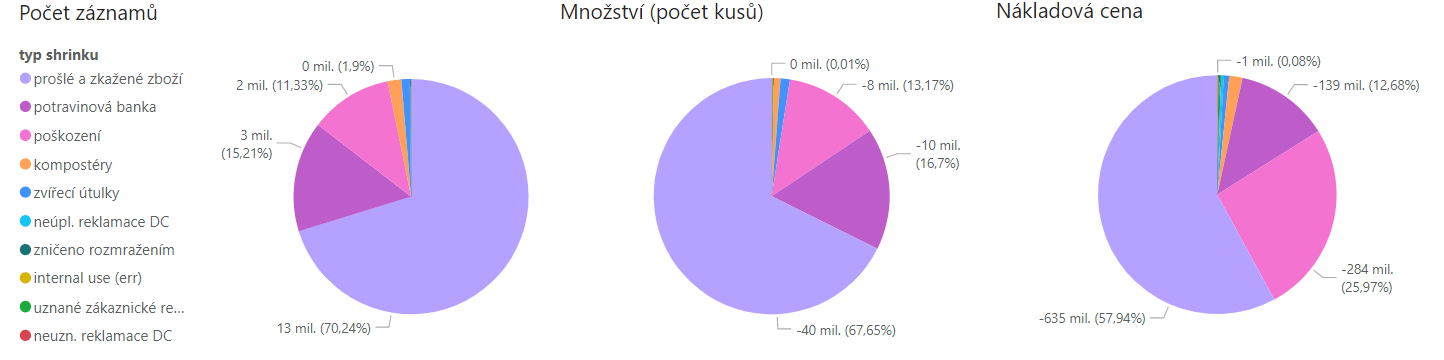
\includegraphics[width=\textwidth]{obrazky/grafy/Graf_celkem-D.png}
    \caption{Zastoupení shrinků typu damage v roce 2022.}
    \label{obr:rok:g:celkemD}
\end{figure}

\subsubsection*{Závislost typu shrinku na čase}

Porovnala jsem množství zaznamenaných shrinků v závislosti na dnech v týdnu, porovnání lze vidět na obr. \ref*{obr:rok:g:tydenD}. Jednotlivé typy jsou zastoupeny analogicky jako v souhrnném přehledu shrinků za jeden rok, tj. prošlé zboží, zboží zaslané do potravinové banky a poškozené zboží. Počty záznamů pro všechny dny jsou v rozmezí $1{,}6$ až $1{,}9$ milionů záznamů  za jeden rok. %!!! nebylo by lepsi tam dat prumer souctu za mesic za cely rok???

\begin{figure}[hbtp!]
    \centering
    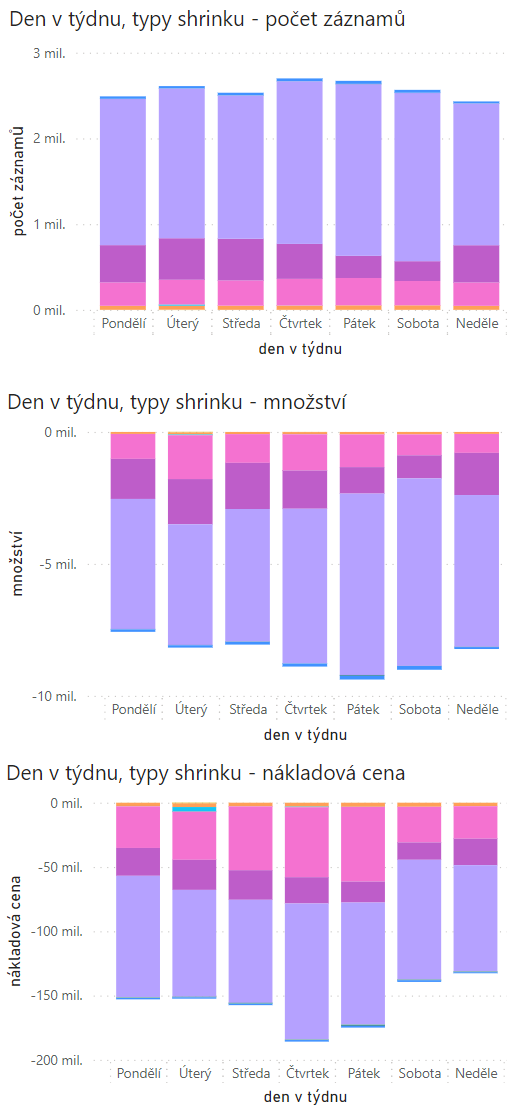
\includegraphics[width=0.5\textwidth]{obrazky/grafy/Grad_dny_tyden-D.png}
    \caption{Zastoupení shrinků typu damage v závislosti na dni v týdnu (údaje pro rok 2022).}
    \label{obr:rok:g:tydenD}
\end{figure}

\begin{figure}[hbtp!]
    \centering
    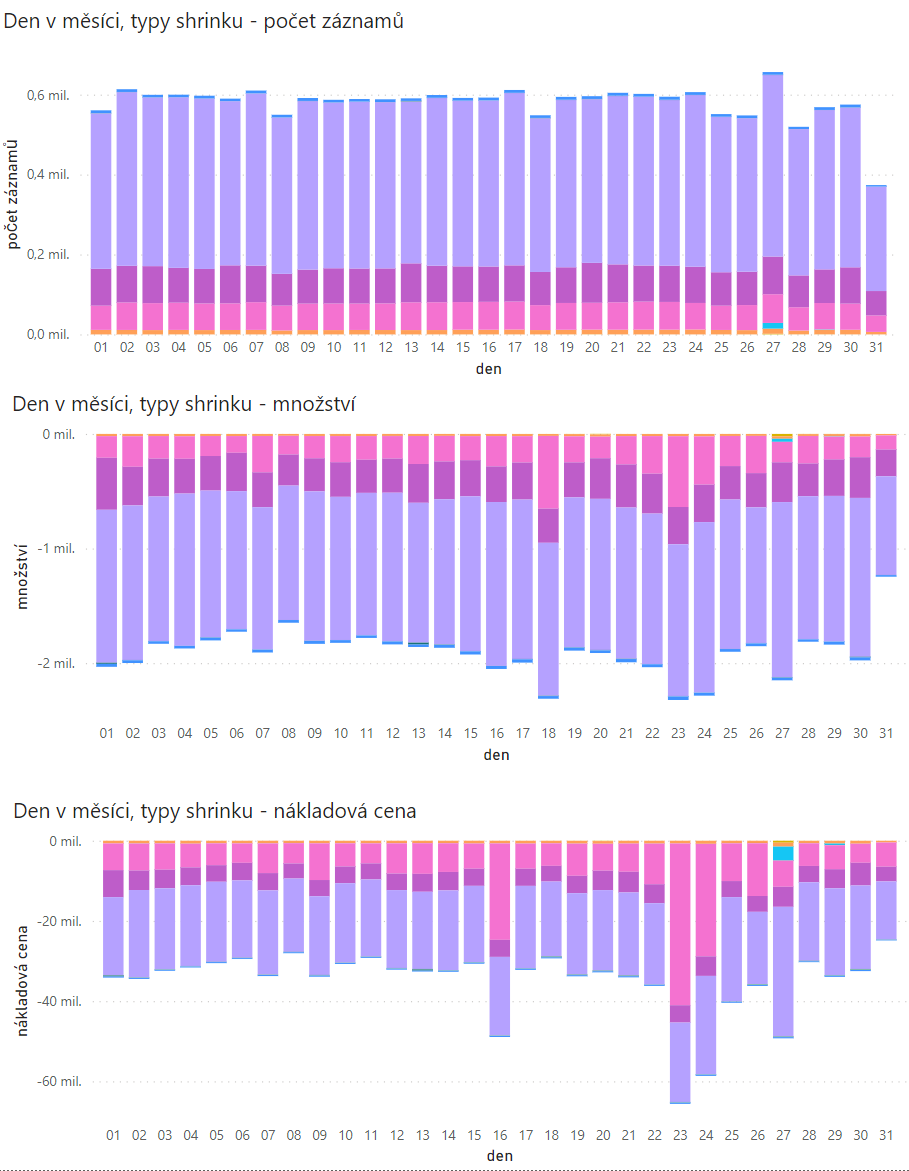
\includegraphics[width=\textwidth]{obrazky/grafy/Grad_dny_mesic-D.png}
    \caption{Zastoupení shrinků typu damage v závislosti na dni v měsíci (údaje pro rok 2022).}
    \label{obr:rok:g:mesicD}
\end{figure}

\subsubsection*{Závislost typu shrinku na hlavní kategorii zboží}

Přehled zastoupení shrinků v závislosti na kategorii zboží je znázorněn na obr. \ref{} %!!! doplnit obrazek (tri vedle sebe  grafiky).
Kategorií, u které bylo evidováno nejvíce damage shrinků je kategorie produktů \emph{superfresh}. Celkově za rok 2022 ztracené náklady byly v hodnotě $0{,}6$ miliardy korun.
V rámci této kategorie je opět nejčastější příčinou odpisu zboží překročená doba expirace, u \emph{superfresh} produktů spíše viditelné zkažení zboží, neboť část \emph{superfresh} produktů nemá uvedenou dobu spotřeby. Druhý nejčastější shrink je shrink označující potravinovou banku. Zbylé shrinky jsou pro tuto kategorii již méně zastoupeny. 
Kategorie \emph{superfresh} má největší zastoupení většiny typů shrinků nad ostatními kategoriemi - přehled zastoupení jednotlivých shrinků odděleně je na obr. \ref{} %!!! udělat obrazek kde budou vedle sebe grafiký pro kazdy shrink
Druhá kategorie, která má nejvíce zaznamenaných shrinků, je kategorie \emph{fresh food} 



\subsubsection*{Závislost typu shrinku na typu prodejny}


